\section{Segmentation of land zones}
\label{sec:segmentation}

\WIP{
now fundamentals of training were laid out and dataset is prepared. this section focuses on implementing reference architectures from section \ref{sec:ref_archs}. Each model first trained and evaluated with original hyperparameters from authors of papers. afterwards, slight modifications are applied to each model, to find potential optimizations suitable for the given task.

All implementations done in Python with popular Keras framework and TensorFlow backend. Was chosen because well established framework with extensive tooling, lots of documentation online and a great community. Also proven to be production-ready and used successfully by broad variety of companies for all kinds of tasks. case studies can be found at \url{https://www.tensorflow.org/about/case-studies}. more information on tools and hardware is to be found in appendix \ref{app:tools_hardware}.
}

\subsection{Preparing the training and test dataset}
\label{sec:prepare_train_test}
\WIP{
\cite{DLbook16}[p.~101f]
before training we have to think about how to evaluate the models afterwards. goal is to have a model that is able to generalize, meaning it should work on data that is has not seen during training. Therefore, dataset is split into two disjoint sets of data, one called the \emph{training set} and the other called \emph{test set}. During training, only data from the training set is presented to the model. afterwards, performance is measured against the test set. That way the metrics provide a more objective view on the performance.

\cite{DLbook16}[p.~119]
test set should not be used to make any choices about the model. To optimize hyperparameters for the model, another split of training data, called \emph{validation set} is introduced. Training set is used to learn parameters, validation set is used to estimate generalization error without consulting the test set. Only after hyperparameters and model weights are optimized all the way, test set is used to measure overall performance of the model.

\cite{val_split18}
There are many ways to pick data for test and validation set. An insight into common techniques is provided by \cite{val_split18}. For this thesis, test set is selected based on imbalance between categories. For each category choose $10\%$ of samples randomly and add them to test set. This is to achieve fair results taking into account all categories accordingly. Validation set also $10\%$ of training set, but chosen randomly over all samples without considering segmentation categories.

as said in \ref{sec:dataset_considerations}, big imbalance between categories in the dataset. this might lead to unwanted biases while training the model. for examples, if network predicts only forest all the time, accuracy would be around $65\%$ measured over entire dataset. plain number is not too bad, but obviously segmentation predictions would be useless.

there are some techniques to tackle those issues. one approach is to add class weights for calculating the loss function. by doing that, incorrect predictions for some classes can be punished more than others. this will result in the model being optimized in a different way, reducing the predictions for the over-represented classes. However, this was not found to work great with given dataset. all experiments had the models end up to only predict a single class for every pixel.

Another approach was selected as follows. dataset contains huge segments that all belong to same class. it was expected, that this circumstance leads to the models learning that most examples only contain one class instead of learning the differences between classes. because of that, the dataset used for training and validation was reduced by a great margin. Basically, all image files that consist of only one class for every pixel are dropped. on the one hand, this affects class imbalance, because large partitions of forests and agricultural regions are dropped, but mostly small streets and rivers are rather kept. on the other hand, this creates incentives for the models to learn the differences between classes.

% TODO: add table with category distribution of multisegment
}

\subsection{Experiments with U-Net}

\WIP{
U-Net was first architecture to explore and experiment with. Model based on findings of \cite{unet15} and explained in detail in section \ref{sec:unet}. Keras implementation used for this thesis listed in appendix~\ref{app:code}.

input image size was chosen as $572\times 572$ pixels, same as authors used. because no padding used in convolutional layers, label/prediction size is smaller, $388\times 388$ pixels for standard U-Net architecture. architecture was also evaluated with fewer layers, label size respectively larger.

based on original model a few other configurations have been explored. base model called \texttt{U-Net-23D}. Number in the name is number of convolution layers in the model. \texttt{D} at the end if dropout layer is used for regularization. one model trained with class weights, this has \texttt{CW} at the end of name.

\ref{fig:unet_train_metrics} shows training metrics from unet models. plots are loss, categorical accuracy, mean iou per epoch calculated from validation set during training. validation data was not used for updating weights, only for evaluation. thus, the numbers provide good evidence of models generalization ability.

clearly visible that \texttt{U-Net-23D-CW} did not perform well. Training was stopped after 5 epochs, because no improvement. loss was lower than other models, this is natural, because weigts reduce the loss for some classes, but does not increase it for the others. also other metrics show that this model performed very poorly.

for \texttt{U-Net-18D} first few epochs show improvement on all metrics. level out after around 5 epochs, then only minor changes. could be that the model reached its capacity. fewer conv layers means less parameters and thus reduced ability to learn and generalize features. end up with $61\%$ categorical accuracy and $21.7\%$ mean IoU.

best results yield model with full $23$ convolution layers. with dropout, model learns a bit faster. after 20 epochs both variants arrive at around $74\%$ categorical accuracy and $42.2\%$ mean iou.

}

\begin{figure}
    \newcommand{\UnetMetricsImageWidth}{0.32\textwidth}
    \centering
            \begin{scaletikzpicturetowidth}{\textwidth}
\begin{tikzpicture}[scale=\tikzscale]
    \begin{axis}[
        mark=x,
        cycle list name=mycolorlist,
        name=unetplot1,
        xmin=1, xmax=20,
    ]

    \addplot
    coordinates{
        (1, 1.3805760145187378)
        (2, 1.2029350996017456)
        (3, 1.0258171558380127)
        (4, 0.9140180349349976)
        (5, 0.8663129806518555)
        (6, 0.8311066627502441)
        (7, 0.8023157715797424)
        (8, 0.8315499424934387)
        (9, 0.7800722122192383)
        (10, 0.7648837566375732)
        (11, 0.7714964747428894)
        (12, 0.7677916884422302)
        (13, 0.7400503158569336)
        (14, 0.7427014708518982)
        (15, 0.7341839075088501)
        (16, 0.7475335001945496)
        (17, 0.7335283160209656)
        (18, 0.7399769425392151)
        (19, 0.7249587774276733)
        (20, 0.732405960559845)
    };

    \addplot
    coordinates{
        (1, 1.266666054725647)
        (2, 1.2810273170471191)
        (3, 1.1684550046920776)
        (4, 1.1036863327026367)
        (5, 0.9430841207504272)
        (6, 0.904362142086029)
        (7, 0.8709024786949158)
        (8, 0.8564851880073547)
        (9, 0.8495147228240967)
        (10, 0.8020780682563782)
        (11, 0.8123838305473328)
        (12, 0.8001933693885803)
        (13, 0.7681636810302734)
        (14, 0.7739695906639099)
        (15, 0.7636772394180298)
        (16, 0.7632151246070862)
        (17, 0.7528753876686096)
        (18, 0.746317982673645)
        (19, 0.7447842955589294)
        (20, 0.7457795143127441)
    };

    \addplot
    coordinates{
        (1, 1.2214372158050537)
        (2, 1.1931297779083252)
        (3, 1.1903798580169678)
        (4, 1.1395219564437866)
        (5, 1.1235227584838867)
        (6, 1.1210097074508667)
        (7, 1.1146382093429565)
        (8, 1.1130719184875488)
        (9, 1.1082816123962402)
        (10, 1.1061081886291504)
        (11, 1.1077511310577393)
        (12, 1.1041945219039917)
        (13, 1.1035878658294678)
        (14, 1.1043835878372192)
        (15, 1.1015698909759521)
        (16, 1.1020666360855103)
        (17, 1.1022522449493408)
        (18, 1.1018295288085938)
        (19, 1.1012828350067139)
        (20, 1.0986037254333496)
    };

    \addplot
    coordinates{
        (1, 1.3491429090499878)
        (2, 1.3386428356170654)
        (3, 1.3372877836227417)
        (4, 1.3367230892181396)
        (5, 1.3370440006256104)
    };

    \end{axis}
     \begin{axis}[
        mark=x,
        cycle list name=mycolorlist,
        name=unetplot2,
        at=(unetplot1.right of south east), anchor=left of south west,
        legend style={at={(0.5,-0.25)},anchor=north},
        xmin=1, xmax=20,
    ]

    \addplot
    coordinates{
        (1, 0.33829551935195923)
        (2, 0.501347541809082)
        (3, 0.645989179611206)
        (4, 0.685759425163269)
        (5, 0.7034950852394104)
        (6, 0.7160254120826721)
        (7, 0.7236952781677246)
        (8, 0.7100507020950317)
        (9, 0.728688657283783)
        (10, 0.7320661544799805)
        (11, 0.7301645874977112)
        (12, 0.7307804226875305)
        (13, 0.7398107051849365)
        (14, 0.7392005324363708)
        (15, 0.7434249520301819)
        (16, 0.7352943420410156)
        (17, 0.7410112023353577)
        (18, 0.742379903793335)
        (19, 0.7461361289024353)
        (20, 0.744171679019928)
    };
    \addlegendentry{U-Net-23D}

    \addplot
    coordinates{
        (1, 0.5139918327331543)
        (2, 0.4997938871383667)
        (3, 0.5388210415840149)
        (4, 0.5911301374435425)
        (5, 0.6690385341644287)
        (6, 0.6867047548294067)
        (7, 0.6966053247451782)
        (8, 0.7008607387542725)
        (9, 0.7030636668205261)
        (10 0.7222729325294495)
        (11, 0.7182477712631226)
        (12, 0.719925045967102)
        (13, 0.7313004732131958)
        (14, 0.7299023866653442)
        (15, 0.7342550754547119)
        (16, 0.7329625487327576)
        (17, 0.7349392175674438)
        (18, 0.7385514378547668)
        (19, 0.7386317253112793)
        (20, 0.7358725666999817)
    };
    \addlegendentry{U-Net-23}

    \addplot
    coordinates{
        (1, 0.5371174216270447)
        (2, 0.5497292876243591)
        (3, 0.5471416711807251)
        (4, 0.5873233675956726)
        (5, 0.6028231382369995)
        (6, 0.6036145091056824)
        (7, 0.6062009930610657)
        (8, 0.6073462963104248)
        (9, 0.6079839468002319)
        (10 0.6088585257530212)
        (11, 0.60825514793396)
        (12, 0.6091040968894958)
        (13, 0.609974205493927)
        (14, 0.6084813475608826)
        (15, 0.609819769859314)
        (16, 0.6098917722702026)
        (17, 0.6100775003433228)
        (18, 0.6097120046615601)
        (19, 0.6102020740509033)
        (20, 0.6107391715049744)
    };
    \addlegendentry{U-Net-18D}

    \addplot
    coordinates{
        (1, 0.35418376326560974)
        (2, 0.3636733293533325)
        (3, 0.35418376326560974)
        (4, 0.3549674451351166)
        (5, 0.3638293445110321)
    };
    \addlegendentry{U-Net-28D}

    % TODO: there are marks missing, check that
    \end{axis}

    \begin{axis}[
        mark=x,
        cycle list name=mycolorlist,
        at=(unetplot2.right of south east), anchor=left of south west,
        xmin=1, xmax=20,
    ]

    \addplot
    coordinates{
        (1, 0.05638260766863823)
        (2, 0.14802682399749756)
        (3, 0.26493558287620544)
        (4, 0.3173089921474457)
        (5, 0.34128832817077637)
        (6, 0.35409560799598694)
        (7, 0.3660319149494171)
        (8, 0.3550480306148529)
        (9, 0.3808368742465973)
        (10, 0.38574960827827454)
        (11, 0.38261398673057556)
        (12, 0.389729768037796)
        (13, 0.39931049942970276)
        (14, 0.3989291489124298)
        (15, 0.4041154682636261)
        (16, 0.40584757924079895)
        (17, 0.4110846519470215)
        (18, 0.4177403450012207)
        (19, 0.4257056713104248)
        (20, 0.4225998818874359)
    };

    \addplot
    coordinates{
        (1, 0.14475272595882416)
        (2, 0.13903780281543732)
        (3, 0.15666361153125763)
        (4, 0.2455795556306839)
        (5, 0.3087078332901001)
        (6, 0.3261967897415161)
        (7, 0.34233176708221436)
        (8, 0.3468801975250244)
        (9, 0.3550216257572174)
        (10, 0.37385615706443787)
        (11, 0.37024033069610596)
        (12, 0.3713560998439789)
        (13, 0.3893120288848877)
        (14, 0.3913959562778473)
        (15, 0.39039942622184753)
        (16, 0.4139955937862396)
        (17, 0.4096660614013672)
        (18, 0.41300487518310547)
        (19, 0.4125426113605499)
        (20, 0.42267632484436035)
    };

    \addplot
    coordinates{
        (1, 0.15161080658435822)
        (2, 0.1566145420074463)
        (3, 0.15519315004348755)
        (4, 0.1986483931541443)
        (5, 0.21347923576831818)
        (6, 0.2152184098958969)
        (7, 0.21574155986309052)
        (8, 0.21671517193317413)
        (9, 0.2158752679824829)
        (10, 0.21583761274814606)
        (11, 0.21597759425640106)
        (12, 0.21608270704746246)
        (13, 0.21780423820018768)
        (14, 0.21527351438999176)
        (15, 0.21591143310070038)
        (16, 0.21773125231266022)
        (17, 0.21799170970916748)
        (18, 0.21698665618896484)
        (19, 0.21827103197574615)
        (20, 0.21748535335063934)
    };

    \addplot
    coordinates{
        (1, 0.059030625969171524)
        (2, 0.06061220541596413)
        (3, 0.059030625969171524)
        (4, 0.059161242097616196)
        (5, 0.060638222843408585)
    };

    \end{axis}

    \node[align=center] at (3.3, -0.65) {\tiny loss};
    \node[align=center] at (11, -0.65) {\tiny cat. accuracy};
    \node[align=center] at (19, -0.65) {\tiny mean IoU};
\end{tikzpicture}
\end{scaletikzpicturetowidth}

    \caption{Training metrics of different variations of U-Net}
    \label{fig:unet_train_metrics}
\end{figure}

\begin{figure}
    \newcommand{\UnetPredictionsImageWidth}{0.18\textwidth}
    \centering

    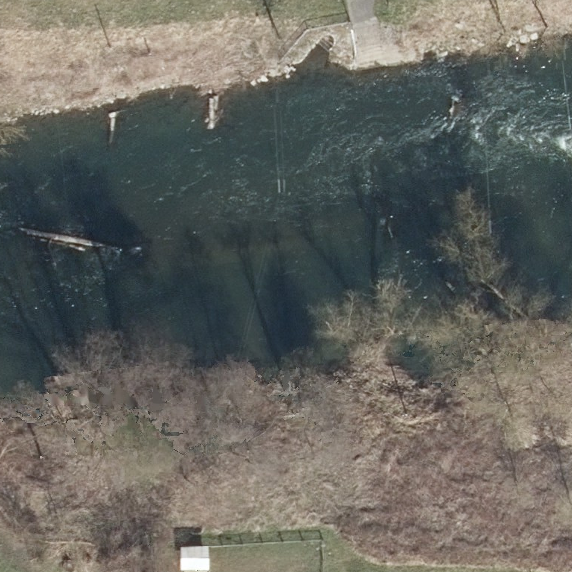
\includegraphics[width=\UnetPredictionsImageWidth]{images/unet/82607-image} \hfill
    
\includegraphics[width=\UnetPredictionsImageWidth]{images/unet/82607-label} \hfill
    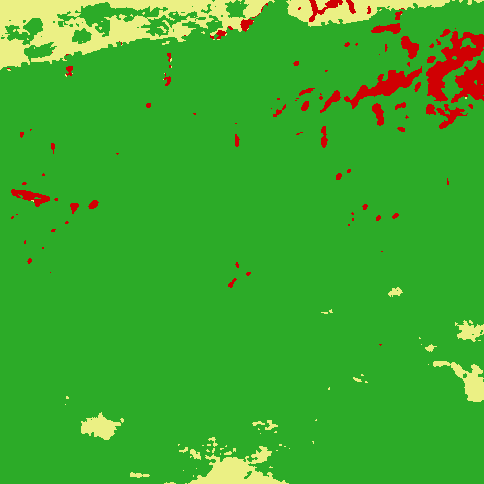
\includegraphics[width=\UnetPredictionsImageWidth]{images/unet/unet-18D/82607-prediction} \hfill
    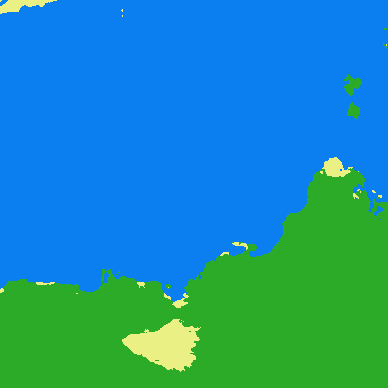
\includegraphics[width=\UnetPredictionsImageWidth]{images/unet/unet-23/82607-prediction} \hfill
    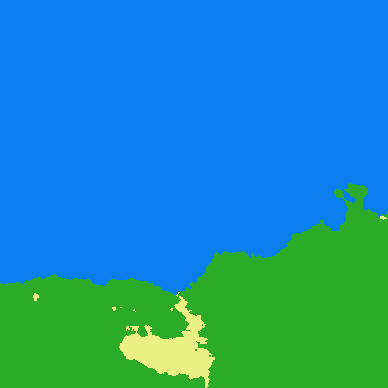
\includegraphics[width=\UnetPredictionsImageWidth]{images/unet/unet-23D/82607-prediction}

    \vspace{3mm}
    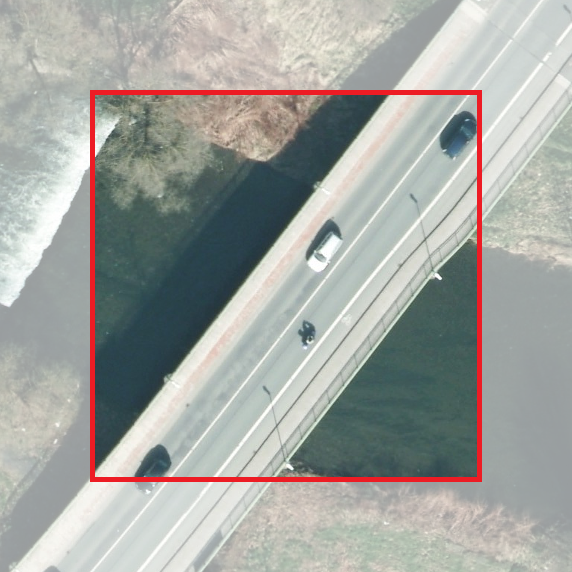
\includegraphics[width=\UnetPredictionsImageWidth]{images/unet/104483-image} \hfill
    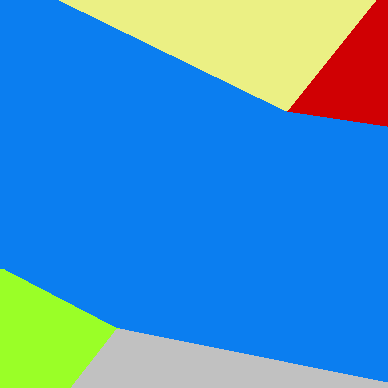
\includegraphics[width=\UnetPredictionsImageWidth]{images/unet/104483-label} \hfill
    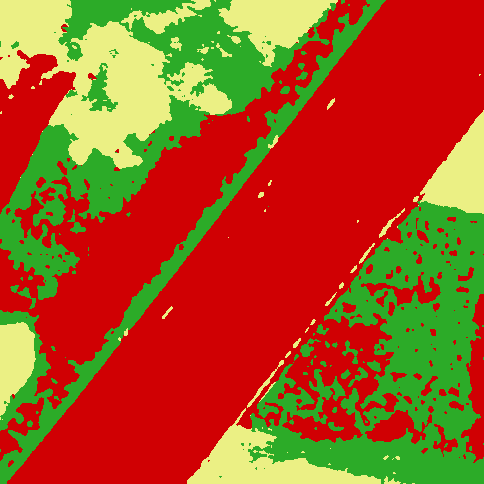
\includegraphics[width=\UnetPredictionsImageWidth]{images/unet/unet-18D/104483-prediction} \hfill
    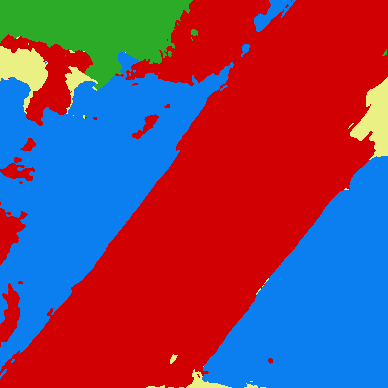
\includegraphics[width=\UnetPredictionsImageWidth]{images/unet/unet-23/104483-prediction} \hfill
    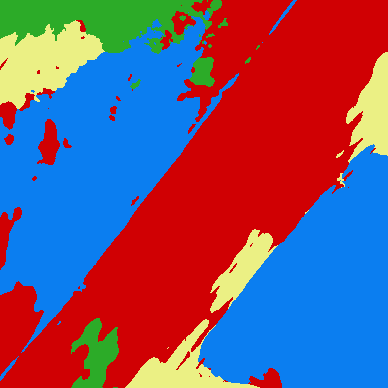
\includegraphics[width=\UnetPredictionsImageWidth]{images/unet/unet-23D/104483-prediction}

    \vspace{3mm}
    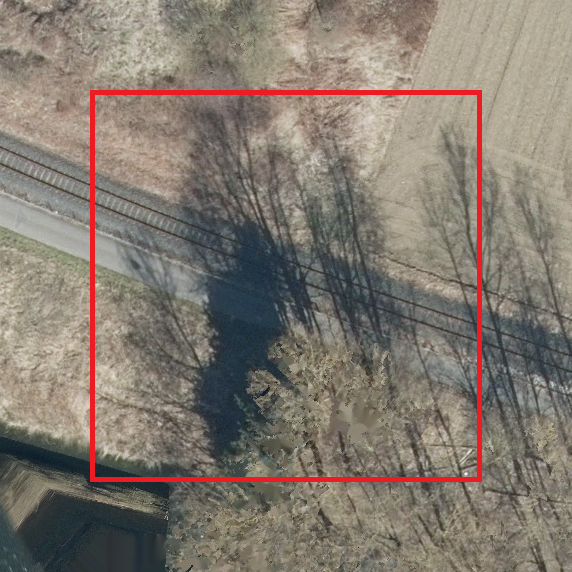
\includegraphics[width=\UnetPredictionsImageWidth]{images/unet/114975-image} \hfill
    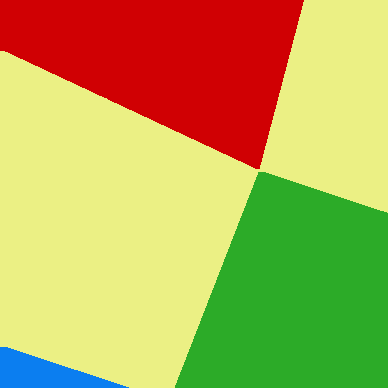
\includegraphics[width=\UnetPredictionsImageWidth]{images/unet/114975-label} \hfill
    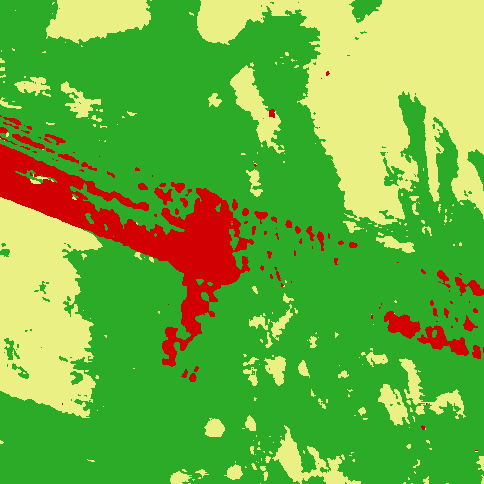
\includegraphics[width=\UnetPredictionsImageWidth]{images/unet/unet-18D/114975-prediction} \hfill
    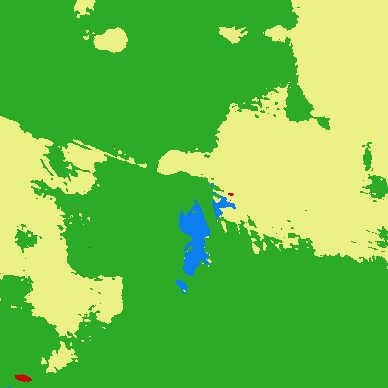
\includegraphics[width=\UnetPredictionsImageWidth]{images/unet/unet-23/114975-prediction} \hfill
    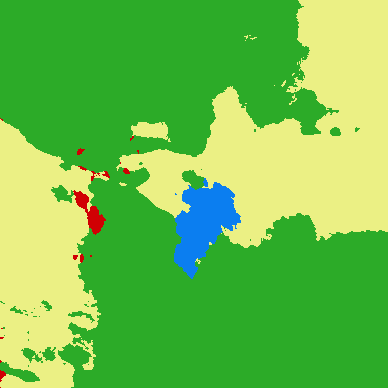
\includegraphics[width=\UnetPredictionsImageWidth]{images/unet/unet-23D/114975-prediction}

    \vspace{3mm}
    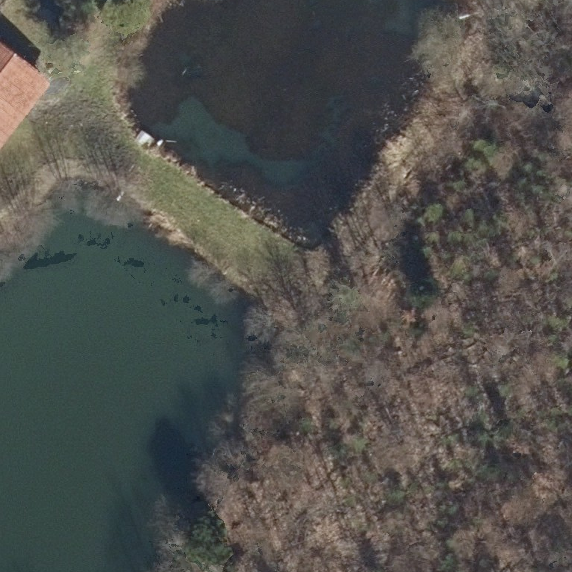
\includegraphics[width=\UnetPredictionsImageWidth]{images/unet/138625-image} \hfill
    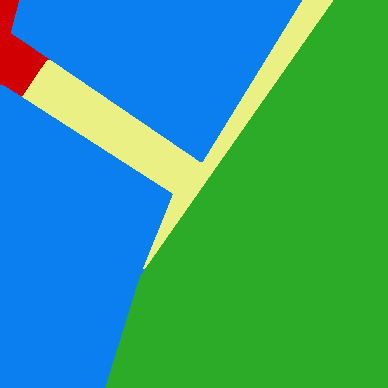
\includegraphics[width=\UnetPredictionsImageWidth]{images/unet/138625-label} \hfill
    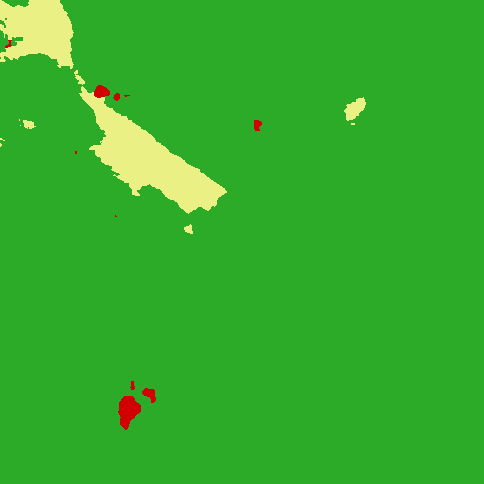
\includegraphics[width=\UnetPredictionsImageWidth]{images/unet/unet-18D/138625-prediction} \hfill
    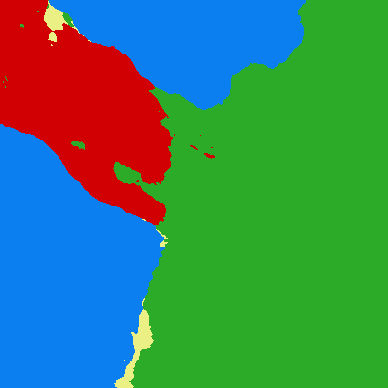
\includegraphics[width=\UnetPredictionsImageWidth]{images/unet/unet-23/138625-prediction} \hfill
    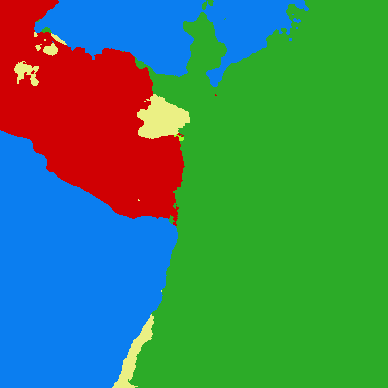
\includegraphics[width=\UnetPredictionsImageWidth]{images/unet/unet-23D/138625-prediction}

    \vspace{3mm}
    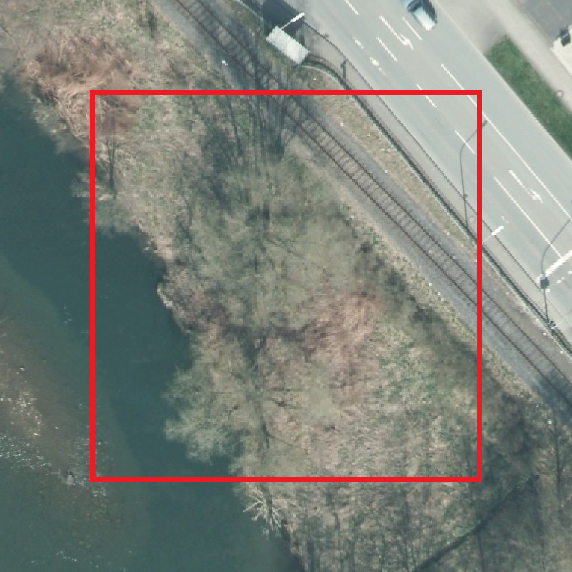
\includegraphics[width=\UnetPredictionsImageWidth]{images/unet/147352-image} \hfill
    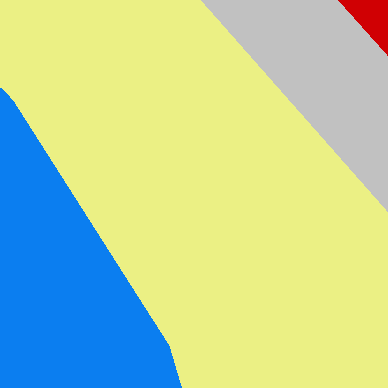
\includegraphics[width=\UnetPredictionsImageWidth]{images/unet/147352-label} \hfill
    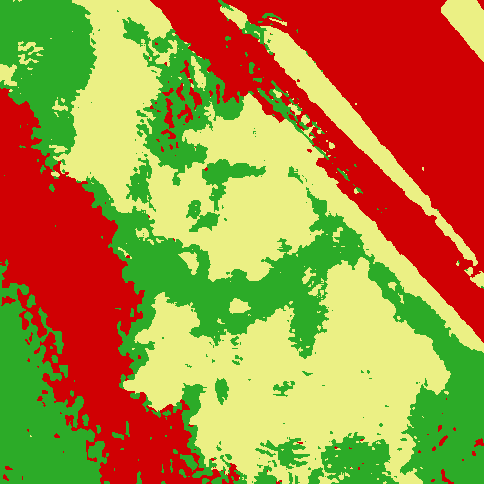
\includegraphics[width=\UnetPredictionsImageWidth]{images/unet/unet-18D/147352-prediction} \hfill
    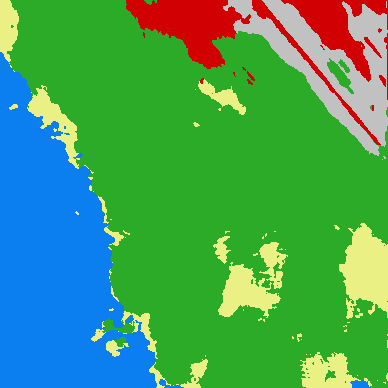
\includegraphics[width=\UnetPredictionsImageWidth]{images/unet/unet-23/147352-prediction} \hfill
    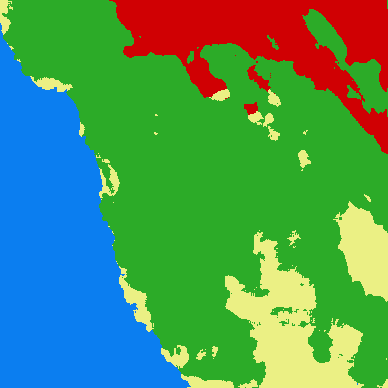
\includegraphics[width=\UnetPredictionsImageWidth]{images/unet/unet-23D/147352-prediction}

    \begin{tikzpicture}
        \node[align=center] at (-1.2, 0) {\tiny Input};
        \node[align=center] at (2.0, 0) {\tiny Ground Truth};
        \node[align=center] at (5.0, 0) {\tiny U-Net-18D};
        \node[align=center] at (8.1, 0) {\tiny U-Net-23};
        \node[align=center] at (11, 0) {\tiny U-Net-23D};
    \end{tikzpicture}
    \caption{Selected predictions of different variantions of U-Net}
    \label{fig:unet_prediction_images}
\end{figure}





\subsection{Experiments with FC-DenseNet}
\WIP{
\begin{itemize}
    \item show the architectures of all FC-DenseNet models
    \item describe the idea behind the architectural decisions
\end{itemize}
}

\begin{figure}
    \newcommand{\DensenetPredictionsImageWidth}{0.13\textwidth}
    \centering

    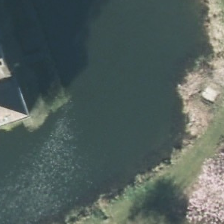
\includegraphics[width=\DensenetPredictionsImageWidth]{images/densenet/101444-image} \hfill
    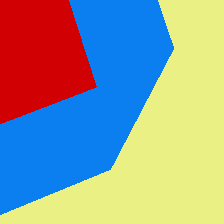
\includegraphics[width=\DensenetPredictionsImageWidth]{images/densenet/101444-label} \hfill
    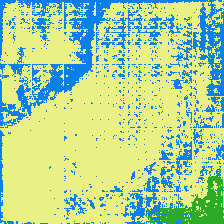
\includegraphics[width=\DensenetPredictionsImageWidth]{images/densenet/densenet-103D/101444-prediction} \hfill
    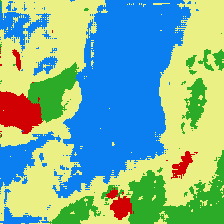
\includegraphics[width=\DensenetPredictionsImageWidth]{images/densenet/densenet-103CD/101444-prediction} \hfill
    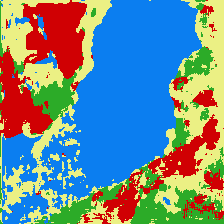
\includegraphics[width=\DensenetPredictionsImageWidth]{images/densenet/densenet-103/101444-prediction} \hfill
    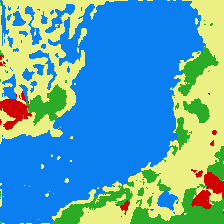
\includegraphics[width=\DensenetPredictionsImageWidth]{images/densenet/densenet-67D/101444-prediction}

    \vspace{3mm}
    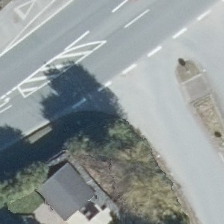
\includegraphics[width=\DensenetPredictionsImageWidth]{images/densenet/291991-image} \hfill
    
\includegraphics[width=\DensenetPredictionsImageWidth]{images/densenet/291991-label} \hfill
    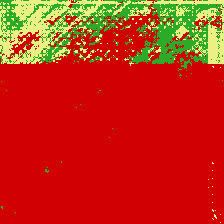
\includegraphics[width=\DensenetPredictionsImageWidth]{images/densenet/densenet-103D/291991-prediction} \hfill
    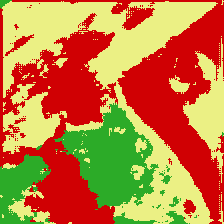
\includegraphics[width=\DensenetPredictionsImageWidth]{images/densenet/densenet-103CD/291991-prediction} \hfill
    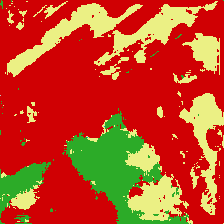
\includegraphics[width=\DensenetPredictionsImageWidth]{images/densenet/densenet-103/291991-prediction} \hfill
    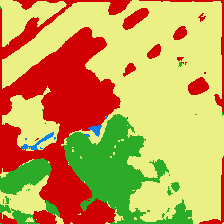
\includegraphics[width=\DensenetPredictionsImageWidth]{images/densenet/densenet-67D/291991-prediction}

    \vspace{3mm}
    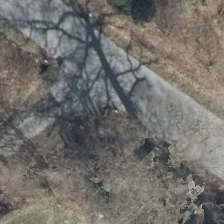
\includegraphics[width=\DensenetPredictionsImageWidth]{images/densenet/436897-image} \hfill
    
\includegraphics[width=\DensenetPredictionsImageWidth]{images/densenet/436897-label} \hfill
    
\includegraphics[width=\DensenetPredictionsImageWidth]{images/densenet/densenet-103D/436897-prediction} \hfill
    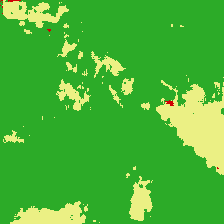
\includegraphics[width=\DensenetPredictionsImageWidth]{images/densenet/densenet-103CD/436897-prediction} \hfill
    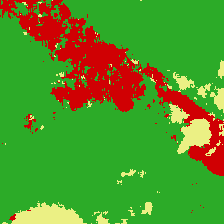
\includegraphics[width=\DensenetPredictionsImageWidth]{images/densenet/densenet-103/436897-prediction} \hfill
    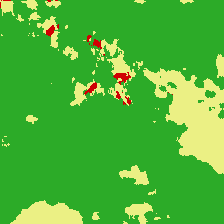
\includegraphics[width=\DensenetPredictionsImageWidth]{images/densenet/densenet-67D/436897-prediction}

    \vspace{3mm}
    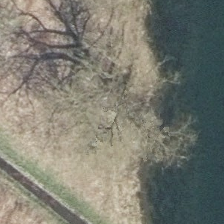
\includegraphics[width=\DensenetPredictionsImageWidth]{images/densenet/626312-image} \hfill
    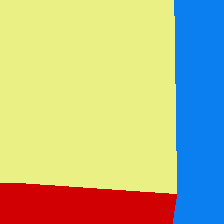
\includegraphics[width=\DensenetPredictionsImageWidth]{images/densenet/626312-label} \hfill
    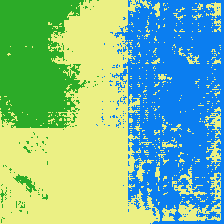
\includegraphics[width=\DensenetPredictionsImageWidth]{images/densenet/densenet-103D/626312-prediction} \hfill
    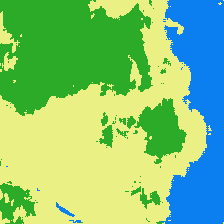
\includegraphics[width=\DensenetPredictionsImageWidth]{images/densenet/densenet-103CD/626312-prediction} \hfill
    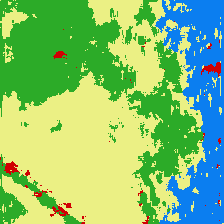
\includegraphics[width=\DensenetPredictionsImageWidth]{images/densenet/densenet-103/626312-prediction} \hfill
    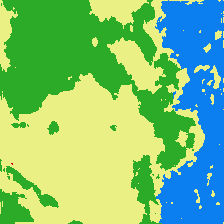
\includegraphics[width=\DensenetPredictionsImageWidth]{images/densenet/densenet-67D/626312-prediction}

    \vspace{3mm}
    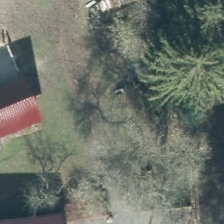
\includegraphics[width=\DensenetPredictionsImageWidth]{images/densenet/768909-image} \hfill
    \includegraphics[width=\DensenetPredictionsImageWidth]{images/densenet/768909-label} \hfill
    \includegraphics[width=\DensenetPredictionsImageWidth]{images/densenet/densenet-103D/768909-prediction} \hfill
    \includegraphics[width=\DensenetPredictionsImageWidth]{images/densenet/densenet-103CD/768909-prediction} \hfill
    \includegraphics[width=\DensenetPredictionsImageWidth]{images/densenet/densenet-103/768909-prediction} \hfill
    \includegraphics[width=\DensenetPredictionsImageWidth]{images/densenet/densenet-67D/768909-prediction}

    \begin{tikzpicture}
        \node[align=center] at (-1.2, 0) {\tiny Input};
        \node[align=center] at (2.0, 0) {\tiny Ground Truth};
        \node[align=center] at (5.0, 0) {\tiny U-Net-18D};
        \node[align=center] at (8.1, 0) {\tiny U-Net-23};
        \node[align=center] at (11, 0) {\tiny U-Net-23D};
    \end{tikzpicture}
    \caption{Selected predictions of different variantions of FC-DenseNet}
    \label{fig:densenet_prediction_images}
\end{figure}

\subsection{Experiments with W-Net}
\WIP{
\begin{itemize}
    \item show the architectures of all W-Net models
    \item describe the idea behind the architectural decisions
\end{itemize}
}

\subsection{Discussion}
\WIP{
\begin{itemize}
    \item have a look at the segments that were found by the NN
    \item show segmentation results of large areas
    \item compare segments to the real landscape in the dataset
    \item discuss practical use of those results for identifying emergency landing fields
    \item evaluate results and assess which data to use for the vegetation analysis
\end{itemize}
}

\newpage
